From the given information
\begin{align}
	\vec{u} = -\myvec{2\\2}, \, \vec{A} &= \myvec{4\\5}\\
\implies	\norm{\vec{A}}^2+2\vec{u}^\top\vec{A}+f &= 0\\
\implies	f = -\norm{\vec{A}}^2 - 2\vec{u}^\top\vec{A}
	&= -5
\end{align}
Hence the equation of circle is 
\begin{align}
	\norm{\vec{x}}^2+2\myvec{-2&-2}\vec{x}-5 = 0 	
\end{align}
See 
\figref{fig:chapters/11/11/1/14/1}.
\begin{figure}[H]
\centering
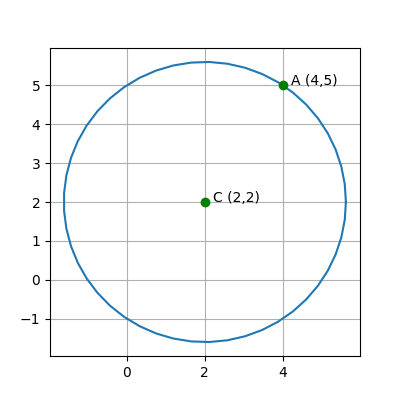
\includegraphics[width=0.75\columnwidth]{chapters/11/11/1/14/figs/fig.png}
\caption{}
\label{fig:chapters/11/11/1/14/1}
\end{figure}






